\documentclass{article}
\usepackage[T1]{fontenc}
\usepackage{lmodern}
\usepackage{graphicx}
\usepackage{amsmath,amssymb}
\usepackage[a4paper,margin=2cm]{geometry}
\usepackage[absolute,overlay]{textpos}
\setlength{\TPHorizModule}{1mm}
\setlength{\TPVertModule}{1mm}
\usepackage[indonesian]{babel}
\usepackage{hyperref}
\setlength{\emergencystretch}{2em}
% unit: Halaman 15

\begin{document}

% === Halaman 15 (llm) ===

Contoh: Alice dan Bob menyepakati $p = 353$ dan $g = 3$ ( $3 < 353$, dan $3$ adalah akar primitif $353$)

\begin{enumerate}
    \item Alice memilih $a = 97$ dan menghitung
    \[ A = g^a \pmod p = 3^{97} \pmod{353} = 40 \]
    Alice mengirim $A$ kepada Bob.
    \item Bob memilih $b = 233$ dan menghitung
    \[ B = g^b \pmod p = 3^{233} \pmod{353} = 248 \]
    Bob mengirim $B$ kepada Alice.
    \item Alice menghitung kunci rahasia $K$,
    \[ K = B^a \pmod p = 248^{97} \pmod{353} = 160 \]
    \item Bob menghitung kunci rahasia $K$,
    \[ K = A^b \pmod p = 40^{233} \pmod{353} = 160 \]
\end{enumerate}

\vspace{30mm}

Jadi, Alice dan Bob sekarang sudah mempunyai kunci rahasia yang sama, yaitu $K = 160$. Mereka dapat menggunakan $K$ sebagai kunci enkripsi dan dekripsi pesan dengan algoritma kunci simetri.

\begin{center}
    Rinaldi M/II4020 Kriptografi
\end{center}

% deskripsi: Diagram alur pertukaran kunci Diffie-Hellman antara Alice dan Bob, menunjukkan pengiriman parameter g, p dan nilai A, B untuk menghitung kunci rahasia K.
% bbox normalisasi: [0.5200, 0.3400, 0.9700, 0.7300]
\begin{textblock*}{94.50mm}(109.20mm,100.98mm)
\noindent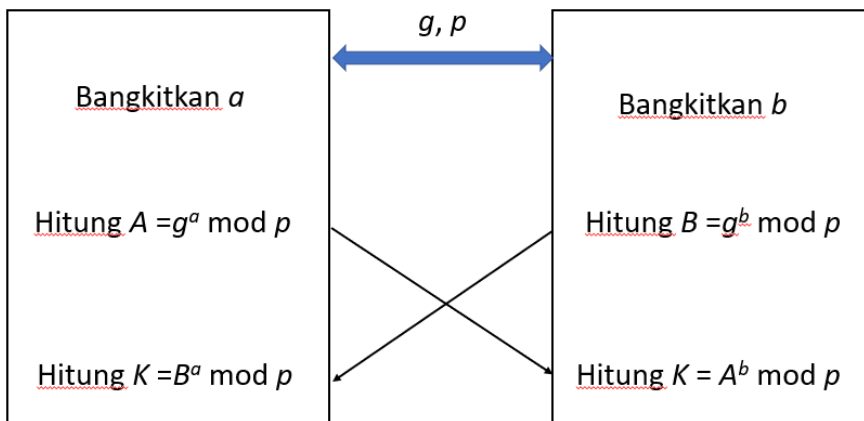
\includegraphics[width=94.50mm,height=115.83mm]{../../images/llm/page_015_img_01.png}%
\end{textblock*}

\end{document}
